\documentclass[11pt]{article}
\usepackage{latexsym}
\usepackage{amsmath}
\usepackage{amssymb}
\usepackage{amsthm}
\usepackage{epsfig}
\usepackage[tight]{subfigure}

\usepackage{amsmath}

\DeclareMathOperator*{\minimize}{min}
\DeclareMathOperator*{\maximize}{max}

\usepackage{algorithm}
 %on linux you may need to run sudo apt-get install texlive-full to install algorithm.sys
\usepackage{algorithmic}

\usepackage{verbatim}

\newcommand{\handout}[5]{
  \noindent
  \begin{center}
  \framebox{
    \vbox{
      \hbox to 5.78in { {#1} \hfill #2 }
      \vspace{4mm}
      \hbox to 5.78in { {\Large \hfill #5  \hfill} }
      \vspace{2mm}
      \hbox to 5.78in { {\em #3 \hfill #4} }
    }
  }
  \end{center}
  \vspace*{4mm}
}

\newcommand{\lecture}[5]{\handout{#1}{#2}{#3}{#4}{#5}}
\newcommand{\collision}[0]{\mathrm{collision}}
\newcommand{\nocollision}[0]{\overline{\collision}}

\newcommand*{\QED}{\hfill\ensuremath{\square}}

\newtheorem{theorem}{Theorem}
\newtheorem{corollary}[theorem]{Corollary}
\newtheorem{lemma}[theorem]{Lemma}
\newtheorem{observation}[theorem]{Observation}
\newtheorem{proposition}[theorem]{Proposition}
\newtheorem{definition}[theorem]{Definition}
\newtheorem{claim}[theorem]{Claim}
\newtheorem{fact}[theorem]{Fact}
\newtheorem{assumption}[theorem]{Assumption}
\newtheorem{note}[theorem]{Note}

% 1-inch margins, from fullpage.sty by H.Partl, Version 2, Dec. 15, 1988.
\topmargin 0pt
\advance \topmargin by -\headheight
\advance \topmargin by -\headsep
\textheight 8.9in
\oddsidemargin 0pt
\evensidemargin \oddsidemargin
\marginparwidth 0.5in
\textwidth 6.5in

\parindent 0in
\parskip 1.5ex
%\renewcommand{\baselinestretch}{1.25}

\begin{document}

\lecture{Statistical Techniques in Robotics (16-831, S20)}{Lecture \#21
  (Wednesday, April 6)}{Lecturer: Kris Kitani}{Scribes: Xiaofeng Guo}{Policy Gradient Methods, Actor-Critic}
  
  
\section{Review}

In the last lectures, we talked about the topic of Function Approximators. In this lecture, we will introduce the Policy-based method: Policy Gradient and hybrid method:Actor-Critic for RL. In this section, we will review the function approximation.



% \begin{algorithm}[H]
% \caption{MC-Control$(\pi, \epsilon, \alpha)$}
% \label{algo:MCpolicy}
% \begin{algorithmic}[1]
% \FOR{$e = 0,...,E$}
% \STATE $\{s^{(t)},a^{(t)},r^{(t)}\}_{t=0}^T \sim \mathcal{E}|\pi$
% \FOR{$t=0,...,T$}
% \STATE $G^{(t)} = \sum_{i=t}^T r^{(i)}$
% \STATE $Q(a^{(t)},s^{(t)}) \leftarrow Q(a^{(t)},s^{(t)}) + \alpha [G^{(t)}-Q(a^{(t)},s^{(t)})]$
% \STATE $\pi(a|s) \leftarrow \frac{\epsilon}{|\mathcal{A}|} + \textbf{1}[a=\arg\max_a Q (a,s^{(t)})](1-\epsilon) \quad \forall{a,s}$
% \ENDFOR
% \ENDFOR 
% \RETURN $\pi$
% \end{algorithmic}
% \end{algorithm}

\subsection{Function Approximation}

If we assume the a finite state and action space, it will lead to a tabular value function and we have multiple different model-free methods based on this assumption. However, when the state space is very large or continuous, we can not represent the value function as the tabular case. Therefore, we need to approximate the value function $V^\pi(s)$ by a parametric function $V_\theta(s)$ so that $V_\theta(s) \approx V^\pi(s)$. We can use multiple different approximators such as linear approximator, neural network, or deep neural network. 

\subsubsection{Value Function Approximation}

To approximate the value function $V^\pi(s)$ by a parametric function $V_\theta(s)$, the goal is to find the optimal $\theta$ 

$$\hat{\theta} = \arg \min_\theta \mathbb{E}_p[(V(s)-V_\theta(s))^2]$$.

We can find the solution using the stochastic gradient descent method:

$$\nabla_\theta \mathcal{L}_\theta \approx -(V(s)-V_\theta(s))\frac{\partial}{\partial \theta} V_\theta(s)$$.

Approximating the gradient requires a return estimator:

$$V(s) = \mathbb{E}[G^{(t)}] \approx G^{(t)}.$$

We can select the estimator or any prediction method we have learned, such as Monte-Carlo, TD, etc. and perform SGD to find the optimal $\theta$.

\subsubsection{Function Approximation for Control}

The function approximation for control is similar as above. By replacing $V(s)$ with $Q(s,a)$, we have the goal is to approximate the value function so that $Q_\theta(s,a) \approx Q^\pi(s,a).$ We have 

$$\hat{\theta} = \arg \min_\theta \mathbb{E}_p[(Q^\pi(s,a)-Q_\theta(s,a))^2]$$.
$$\nabla_\theta \mathcal{L}_\theta \approx -(Q^\pi(s,a)-Q_\theta(s,a))\frac{\partial}{\partial \theta} Q_\theta(s,a)$$.
$$Q^\pi(s,a) \approx G^{(t)}.$$

We can select the estimator or any prediction method we have learned to find the optimal $\theta$.

\section{Summary}
\subsection{Policy Gradient Method}
In this subsection, we will summary the Policy Gradient Method. In valued-based methods, the goal is to estimate the value function and the optimal policy was derived from the value function. Different with that, in policy-based method, we are going to estimate the policy $\pi$ directly without estimating the value function. This class of models is called policy gradient methods. For a parametrized policy $\pi_\theta(a|s)$, we want to optimize its parameter $\theta$ that maximizes the expect accumulative return:

\begin{equation}
\begin{split}
\hat{\theta} &= \arg \max_{\theta} \mathbb{E}_{p_\theta(\zeta)}[\sum_{t=0}^T r^{(t)}]\\
&= \arg \max_{\theta} J(\theta)
\end{split}
\label{equ:obj}
\end{equation}

where
$$p_\theta(\zeta) = p(s^{(0)}) \Pi_{t=0}^T \pi_\theta(a^{(t)}|s^{(t)})p(s^{(t+1)}|s^{(t)},a^{(t)})$$
$$\zeta = \{s^{(0)}, a^{(0)}, s^{(1)}, a^{(1)}, ..., s^{(T)}, a^{(T)}\} $$
$$r^{(t)} \triangleq r(s^{(t+1)},a^{(t)},s^{(t)}).$$
To handle this optimization problem, we will use gradient ascent method to find the optimal $\theta$.

\subsubsection{Gradient Ascent Method}

Here we will use gradient ascent method to solve Equation \ref{equ:obj}. First, we make a linear approximation of the objective function with quadratic regularization:

$$\hat{\theta} = \arg \max_{\theta}\{\alpha(J(\theta')+ \langle\theta-\theta', \nabla_{\theta'} J(\theta') \rangle) - \frac{1}{2}||\theta-\theta'||^2 \}.$$

Optimizing the Lagrangian, we get:

$$\nabla_{\theta} \{ \alpha(J(\theta')+ \langle\theta-\theta', \nabla_{\theta'} J(\theta') \rangle) - \frac{1}{2}||\theta-\theta'||^2 \} = 0$$

$$\Rightarrow \alpha \nabla_{\theta'}J(\theta')-\theta+\theta'=0.$$

Therefore, we get the parameter $\theta$ update equation:

\begin{equation}
\theta \leftarrow \theta' + \alpha \nabla_{\theta'} J(\theta'). 
\label{equ:update_theta}
\end{equation}

Recall that we have:

\begin{equation*}
\begin{split}
J(\theta) &= \mathbb{E}_{p_\theta(\zeta)}[\sum_{t=0}^T r^{(t)}] \\
&= \int_\zeta p_\theta(\zeta)r(\zeta) d\zeta \qquad \text{by definition of expectation.}
\end{split}
\end{equation*}

and
$$r(\zeta) = \sum_{t=0}^{T}(r^{(t)}).$$

Therefore, we have the gradient of objective:

\begin{equation*}
\begin{split}
\nabla_{\theta} J(\theta) & = \nabla_{\theta} \int_\zeta p_\theta(\zeta)r(\zeta)d\zeta \qquad \text{by definition}\\
& = \int_\zeta \nabla_{\theta}p_\theta(\zeta)r(\zeta)d\zeta \qquad \text{linearity of gradient}\\
& = \int_\zeta p_\theta(\zeta) \frac{\nabla_{\theta}p_\theta(\zeta)}{p_\theta(\zeta)}r(\zeta)d\zeta \qquad \text{multiply by one}\\
& = \int_\zeta p_\theta(\zeta)\nabla_\theta \ln p_\theta(\zeta)r(\zeta)d\zeta \qquad \text{derivative of log ‘trick'.}
\end{split}
\end{equation*}

Then, let's take a look at the term $\nabla_\theta \ln p_\theta(\zeta)$. We can decompose it as:

\begin{equation*}
\begin{split}
\nabla_\theta \ln p_\theta(\zeta) &= \nabla_\theta [\ln p(s^{(0)}) + \sum_{t=1}^T \ln \pi_\theta(a^{(t)}|s^{(t)}) + \ln p(s^{(t+1)}|s^{(t)},a^{(t)})]\\
& = \nabla_\theta [\sum_{t=1}^T \ln \pi_\theta(a^{(t)}|s^{(t)})] \qquad \text{only policy is dependent on $\theta$.}
\end{split}
\end{equation*}

Bring it back to the gradient $\nabla_\theta J(\theta)$, we have 

\begin{equation}
\begin{split}
\nabla_{\theta} J(\theta) & = \int_\zeta p_\theta(\zeta)\nabla_\theta \ln p_\theta(\zeta)r(\zeta)d\zeta\\
& = \int_\zeta p_\theta(\zeta)\nabla_\theta(\sum_{t=1}^T \ln \pi_\theta(a^{(t)}|s^{(t)}))r(\zeta)d\zeta \qquad \text{keep only terms dependent on $\theta$} \\
& = \mathbb{E}_{p_\theta(\zeta)}[(\sum_{t=1}^T \nabla_\theta \ln \pi_\theta(a^{(t)}|s^{(t)})) (\sum_{t=1}^T r^{(t)})]
\end{split}
\label{equ:gradient}
\end{equation}
 
We call the term $\nabla_\theta \ln \pi_\theta(a^{(t)}|s^{(t)})$ “eligibility vector” and the term $\sum_{t=1}^T r^{(t)}$ "episodic return". \\

Let's first look at the "eligibility vector". We have
$$\nabla_\theta \ln \pi_\theta(a^{(t)}|s^{(t)}) = \frac{\nabla_\theta  \pi_\theta(a^{(t)}|s^{(t)})}{\pi_\theta(a^{(t)}|s^{(t)})},$$

in which $\nabla_\theta  \pi_\theta(a^{(t)}|s^{(t)})$ represents the change in policy $\pi_\theta$ per unit change in $\theta$ and $\pi_\theta(a^{(t)}|s^{(t)})$ represents the inverse probability weighting. Therefore, the “eligibility vector” shows the weighted sensitivity of the policy to change in parameter. Specifically, low probability actions have bigger gradient and high probability actions have smaller gradient.
  

For the "episodic return", we have $r(\zeta) = \sum_{t=1}^T r^{(t)}$. It shows the goodness of the current policy and the gradient is Weighted by this episodic return. Specifically, a good trajectory (large reward) has a bigger gradient and a bad trajectory (small reward) has a smaller gradient.

Note that it is not practical to sum over all possible trajectories when we calculate the expectation, so we approximate it with samples as Monte-Carlo estimate. Therefore, we have 

\begin{equation}
\begin{split}
\nabla_{\theta} J(\theta) & = \mathbb{E}_{p_\theta(\zeta)}[(\sum_{t=1}^T \nabla_\theta \ln \pi_\theta(a^{(t)}|s^{(t)})) (\sum_{t=1}^T r^{(t)})]\\
&\approx \frac{1}{N} \sum_{n=1}^{N}(\sum_{t=1}^T \nabla_\theta \ln \pi_\theta(a^{(n,t)}|s^{(n,t)}))(\sum_{t=1}^T r^{(n,t)}).
\end{split}
\end{equation}

Therefore, we can compute the parameter update Equation \ref{equ:update_theta}.

\subsubsection{Policy Gradient Algorithms}

Based on the above equations, we get the Monte-Carlo Policy Gradient Algorithm as Algorithm \ref{algo:MCpolicy}.
\begin{algorithm}[H]
\caption{MC-Policy-Gradient$(\pi_\theta,\alpha)$}
\label{algo:MCpolicy}
\begin{algorithmic}[1]
\FOR{$e = 1,...,E$}
\STATE $\{s^{(t)},a^{(t)},r^{(t)}\}_{t=0}^T \sim \mathcal{E}|\pi_\theta $
\STATE $G^{(0)} = \sum_{t=0}^T r^{(t)}$
\FOR{$t=0,...,T$}
\STATE $\theta \leftarrow \theta+\alpha(\nabla_{\theta}\log{\pi_\theta(a^{(t)}|s^{(t)})})(G^{(0)})$
\ENDFOR
\ENDFOR 
\RETURN $\pi_\theta$
\end{algorithmic}
\end{algorithm}

However, there is a problem in Monte-Carlo Policy Gradient Method. Monte-Carlo estimation has zero bias but large variance. There are two ways to reduce its variance. In the first method, we can enforce causality. We made a simple observation that the policy decision at time $t'$ cannot affect past rewards at $t<t’$, which means that the update to the policy at time step $t$ should only depend on future reward. Therefore, when computing the $\nabla_{\theta} J(\theta)$, instead on computing the reward for the entire sequence, we only compute the future reward. Therefore, we have 

\begin{equation*}
\begin{split}
\nabla_{\theta} J(\theta) &\approx \frac{1}{N} \sum_{n=1}^{N}(\sum_{t=0}^T \nabla_\theta \ln \pi_\theta(a^{(n,t)}|s^{(n,t)}))(\sum_{t=0}^T r^{(n,t)})\\
&\approx \frac{1}{N}\sum_{n=1}^{N}\sum_{t=0}^T \nabla_\theta \ln \pi_\theta(a^{(n,t)}|s^{(n,t)}) (\sum_{t'=t}^{T}r^{(n,t')})
\end{split}
\end{equation*}


The other method to reduce the variance is to remove the gradient bias with a baseline offset. We know that the reward values might be very large, which may cause very large gradients. We can adjust the gradient by subtracting some offset b:

$$\nabla_{\theta} J(\theta) = \int_\zeta p_\theta(\zeta)\nabla_\theta \ln p_\theta(\zeta)[r(\zeta)-b]d\zeta.$$

We can prove that this offset will not change the expected gradient as bellows.

\begin{equation*}
\begin{split}
\nabla_{\theta} J(\theta) &=  \int_\zeta p_\theta(\zeta)\nabla_\theta \ln p_\theta(\zeta)[r(\zeta)-b]d\zeta \qquad \text{offset version of the gradient}\\
& = \int_\zeta p_\theta(\zeta)\nabla_\theta \ln p_\theta(\zeta)r(\zeta)d\zeta - \int_\zeta p_\theta(\zeta)\nabla_\theta \ln p_\theta(\zeta)b d\zeta\\
& = \int_\zeta p_\theta(\zeta)\nabla_\theta \ln p_\theta(\zeta)r(\zeta)d\zeta - \int_\zeta p_\theta(\zeta) \frac{\nabla_\theta p_\theta(\zeta)}{p_\theta(\zeta)} b d\zeta \\
& = \int_\zeta p_\theta(\zeta)\nabla_\theta \ln p_\theta(\zeta)r(\zeta)d\zeta - \int_\zeta \nabla_\theta p_\theta(\zeta)b d\zeta \\
& = \int_\zeta p_\theta(\zeta)\nabla_\theta \ln p_\theta(\zeta)r(\zeta)d\zeta - b \nabla_\theta \int_\zeta  p_\theta(\zeta) d\zeta \qquad \text{integral of probability is one}\\
& = \int_\zeta p_\theta(\zeta)\nabla_\theta \ln p_\theta(\zeta)r(\zeta)d\zeta - b \nabla_\theta (1) \qquad \text{derivative of constant is zero}\\
& = \int_\zeta p_\theta(\zeta)\nabla_\theta \ln p_\theta(\zeta)r(\zeta)d\zeta - 0 \qquad \text{get back the original gradient.} 
\end{split}
\end{equation*}


Based on the second method, we can get the Episodic-REINFORCE algorithm as Algorithm \ref{algo:Episodic-REINFORCE}.

\begin{algorithm}[H]
\caption{Episodic-REINFORCE$(\pi_\theta,\alpha)$}
\label{algo:Episodic-REINFORCE}
\begin{algorithmic}[1]
\FOR{$e = 1,...,E$}
\STATE $\{s^{(t)},a^{(t)},r^{(t)}\}_{t=0}^T \sim \mathcal{E}|\pi_\theta $
\STATE $G^{(0)} = \sum_{t=0}^T r^{(t)}$
\FOR{$t=0,...,T$}
\STATE $\theta \leftarrow \theta+\alpha [G^{(0)}-b]\nabla_{\theta}\log{\pi_\theta(a^{(t)}|s^{(t)})}$
\ENDFOR
\ENDFOR 
\RETURN $\pi_\theta$
\end{algorithmic}
\end{algorithm}



Putting these two modifications together, we get the policy gradient algorithm as Algorithm \ref{algo:Policy-Gradient}.

\begin{algorithm}[H]
\caption{Policy-Gradient$(\pi_\theta,\alpha, b)$}
\label{algo:Policy-Gradient}
\begin{algorithmic}[1]
\FOR{$e = 1,...,E$}
\STATE $\{s^{(t)},a^{(t)},r^{(t)}\}_{t=0}^T \sim \mathcal{E}|\pi_\theta $
\FOR{$t=0,...,T$}
\STATE $G^{(t)} = \sum_{i=t}^T r^{(i)}$
\STATE $\theta \leftarrow \theta+\alpha [G^{(t)}-b]\nabla_{\theta}\log{\pi_\theta(a^{(t)}|s^{(t)})}$
\ENDFOR
\ENDFOR 
\RETURN $\pi_\theta$
\end{algorithmic}
\end{algorithm}

To conclude, we summary the pros and cons of 
policy gradient methods. 

\textbf{Pros}: Firstly, it doesn’t require model and learns from interaction. Secondly, it is effective for high-dimensional or continuous action spaces (all methods so far assumed finite 
action space). Next, it can encode prior knowledge when designing policy architecture. Finally, it finds the optimal stochastic policy and naturally explores due to stochasticity. 

\textbf{Cons}: Firstly, the gradient is typically high variance and leads to slow convergence. Secondly, a small step size leads to slow convergence. Next, it typically converges to local minima instead of global 
minima. Finally, it is easy to have exploding or zero gradients.


\subsection{Actor Critic}

We have been discussed about the valued-based method and policy-based method. Here we will discuss the hybrid of them. When the value function estimates are used as the baseline, 
for policy gradient methods, this class of methods is called actor-critic. This is currently the most popular RL approach.
  
Recall that in the policy gradient, we need the entire episode to compute the reward $\sum_{t=1}^T r^{(n,t)}$. However, we can use many prediction algorithms to estimate it so that we don’t need full episodes. For continuous case, we can use function approximation for estimation. Therefore, similar with the form of Equation \ref{equ:gradient}, we get the gradient of objective function:

$$\nabla_{\theta} J(\theta) = \mathbb{E}_{p_\theta(\zeta)}[(\sum_{t=1}^T \nabla_\theta \ln \pi_\theta(a^{(t)}|s^{(t)})) (G_\phi^{(t)})],$$

where $G_\phi^{(t)}$ is the return value estimator, which is also called "Critic". By combining the policy gradient method with different approximate estimation method, we can get different Actor-Critic methods. For example, we can combine policy gradient with Q-MC Prediction and get Q-MC Actor Critic algorithm as Algorithm \ref{algo:Q-MC-Actor-Critic}.



\begin{algorithm}[H]
\caption{Q-MC-Actor-Critic$(\pi_\theta,Q_\phi, \alpha, \beta)$}
\label{algo:Q-MC-Actor-Critic}
\begin{algorithmic}[1]
\FOR{$e = 1,...,E$}
\STATE $\{s^{(t)},a^{(t)},r^{(t)}\}_{t=0}^T \sim \mathcal{E}|\pi_\theta $
\FOR{$t=0,...,T$}
\STATE $G^{(t)} = \sum_{i=t}^T r^{(i)}$
\STATE $\phi \leftarrow \phi + \beta[G^{(t)}-Q_\phi(a^{(t)},s^{(t)})]\nabla Q_\phi(a^{(t)},s^{(t)})$
\STATE $\theta \leftarrow \theta+\alpha \nabla_{\theta}\log{\pi_\theta(a^{(t)}|s^{(t)})} \cdot Q_\phi(a^{(t)},s^{(t)}) $
\ENDFOR
\ENDFOR 
\RETURN $\pi_\theta$
\end{algorithmic}
\end{algorithm}


Similarly, we can get Q-TD Actor Critic algorithm as Algorithm \ref{algo:Q-TD-Actor-Critic}

\begin{algorithm}[H]
\caption{Q-TD-Actor-Critic$(\pi_\theta,Q_\phi, \alpha, \beta)$}
\label{algo:Q-TD-Actor-Critic}
\begin{algorithmic}[1]
\FOR{$e = 1,...,E$}
\STATE $\{s^{(t)},a^{(t)},r^{(t)}\}_{t=0}^T \sim \mathcal{E}|\pi_\theta $
\FOR{$t=0,...,T$}
\STATE $\delta \leftarrow r^{(t)} + Q_\phi(a^{(t+1)},s^{(t+1)})$
\STATE $\phi \leftarrow \phi + \beta[\delta-Q_\phi(a^{(t)},s^{(t)})]\nabla Q_\phi(a^{(t)},s^{(t)})$
\STATE $\theta \leftarrow \theta+\alpha \nabla_{\theta}\log{\pi_\theta(a^{(t)}|s^{(t)})} \cdot Q_\phi(a^{(t)},s^{(t)}) $
\ENDFOR
\ENDFOR 
\RETURN $\pi_\theta$
\end{algorithmic}
\end{algorithm}


Now let's go back and discuss about the offset $b$ in 

$$\nabla_{\theta} J(\theta) = \mathbb{E}_{p_\theta(\zeta)}[(\sum_{t=1}^T \nabla_\theta \ln \pi_\theta(a^{(t)}|s^{(t)})) (\sum_{i=t}^T r^{(i)}-b).$$

Let's denote the term $\sum_{i=t}^T r^{(i)}-b$ as “Adjusted Return". We can derive that the optimal baseline $b$ for policy gradient is the value function $V_\psi(s^{(t)})$ and we can get the optimal adjusted return for the policy gradient:

$$A(a^{(t)},s^{(t)}) = Q_\phi(a^{(t)},s^{(t)}) - V_\psi(s^{(t)}).$$


$A(a^{(t)},s^{(t)})$ is called the "Advantage function". The policy gradient with Advantage function is called the “Advantage Actor-Critic” and we have

$$\nabla_{\theta} J(\theta) = \mathbb{E}_{p_\theta(\zeta)}[(\sum_{t=1}^T \nabla_\theta \ln \pi_\theta(a^{(t)}|s^{(t)})) (\sum_{i=t}^T A_\phi(a,s))].$$

Here we show two Advantage Actor-Critic algorithms as Algorithm \ref{algo:Advantage-MC-Actor-Critic}
 and Algorithm \ref{algo:Advantage-TD-Actor-Critic}.
\begin{algorithm}[H]
\caption{Advantage-MC-Actor-Critic$(\pi_\theta,Q_\phi,V_\psi, \alpha, \beta, \kappa)$}
\label{algo:Advantage-MC-Actor-Critic}
\begin{algorithmic}[1]
\FOR{$e = 1,...,E$}
\STATE $\{s^{(t)},a^{(t)},r^{(t)}\}_{t=0}^T \sim \mathcal{E}|\pi_\theta $
\FOR{$t=0,...,T$}
\STATE $G^{(t)}\leftarrow \sum_{i=t}^T r^{(i)}$
\STATE $\psi \leftarrow \psi + \kappa[G^{(t)}-V_\phi(s^{(t)})]\nabla_\psi V_\psi(s^{(t)})$
\STATE $\phi \leftarrow \phi + \beta[G^{(t)}-Q_\phi(a^{(t)},s^{(t)})]\nabla_\phi Q_\phi(a^{(t)},s^{(t)})$
\STATE $\theta \leftarrow \theta+\alpha [Q_\phi(a^{(t)},s^{(t)})-V_\psi(s^{(t)})] \nabla_{\theta}\log{\pi_\theta(a^{(t)}|s^{(t)})}$
\ENDFOR
\ENDFOR 
\RETURN $\pi_\theta$
\end{algorithmic}
\end{algorithm}




\begin{algorithm}[H]
\caption{Advantage-TD-Actor-Critic$(\pi_\theta,Q_\phi,V_\psi, \alpha, \beta, \kappa)$}
\label{algo:Advantage-TD-Actor-Critic}
\begin{algorithmic}[1]
\FOR{$e = 1,...,E$}
\STATE $\{s^{(t)},a^{(t)},r^{(t)}\}_{t=0}^T \sim \mathcal{E}|\pi_\theta $
\FOR{$t=0,...,T$}
\STATE $\delta_V \leftarrow r^{(t)} + V_\psi (s^{(t+1)})$
\STATE $\psi \leftarrow \psi + \kappa[\delta_V -V_\psi(s^{(t)})]\nabla_\psi V_\psi(s^{(t)})$
\STATE $\delta_Q \leftarrow r^{(t)} + Q_\phi (a^{(t+1)},s^{(t+1)})$
\STATE $\phi \leftarrow \phi + \beta[\delta_Q -Q_\phi(a^{(t)},s^{(t)})]\nabla_\phi Q_\phi(a^{(t)},s^{(t)})$
\STATE $\theta \leftarrow \theta+\alpha [Q_\phi(a^{(t)},s^{(t)})-V_\psi(s^{(t)})] \nabla_{\theta}\log{\pi_\theta(a^{(t)}|s^{(t)})}$
\ENDFOR
\ENDFOR 
\RETURN $\pi_\theta$
\end{algorithmic}
\end{algorithm}


  %\section*{References}
%Include your references here. Please cite any resources you found useful.	
%Populate the refs.bib file or list your references manually. Be consistent in formatting!
\nocite{*}
{
\bibliography{refs}
\bibliographystyle{abbrv}
}


\section{Appendix}

Interestingly, the term 'REINFORCE' comes from the abbreviation of 

$$\text{\textbf{RE}ward \textbf{I}ncrement} = \text{\textbf{N}on-negative \textbf{F}actor} \times \text{\textbf{O}ffset \textbf{R}einforcement} \times \text{\textbf{C}haracteristic \textbf{E}ligibility}.$$

as shown in Figure \ref{fig:REINFORCEMENT}.

\begin{figure}[H]
    \centering
    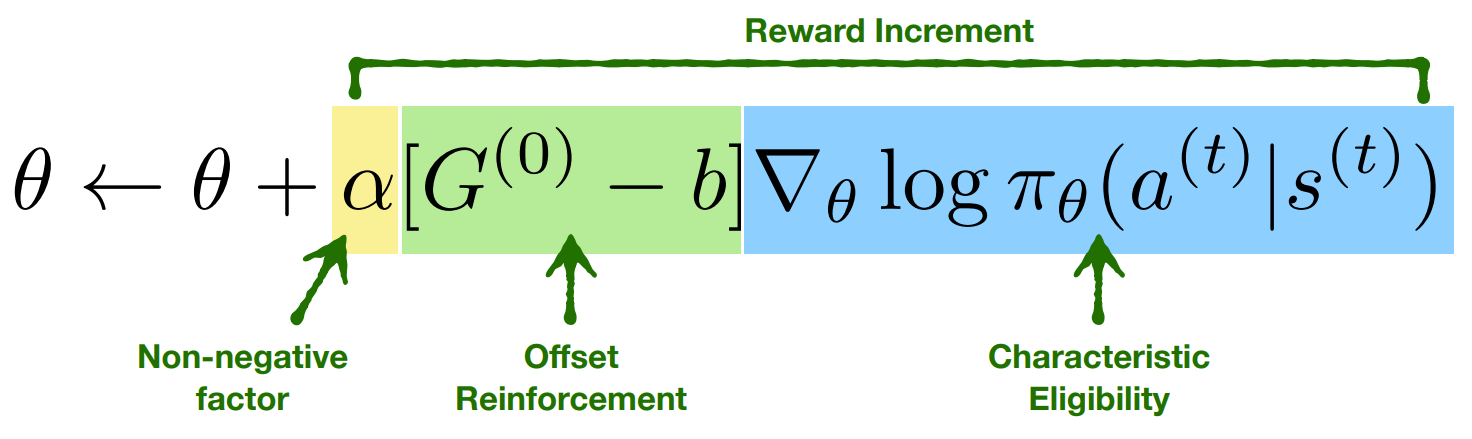
\includegraphics[width = 0.5\linewidth]{1.PNG}
    \caption{'REINFORCE'}
    \label{fig:REINFORCEMENT}
\end{figure}

Figure \ref{fig:stepsize} shows the total reward of REINFORCE without baseline performs with different step size and \ref{fig:converge} shows reduced variance leads to faster convergence \cite{sutton2018reinforcement}.
\begin{figure}[H]
    \centering
    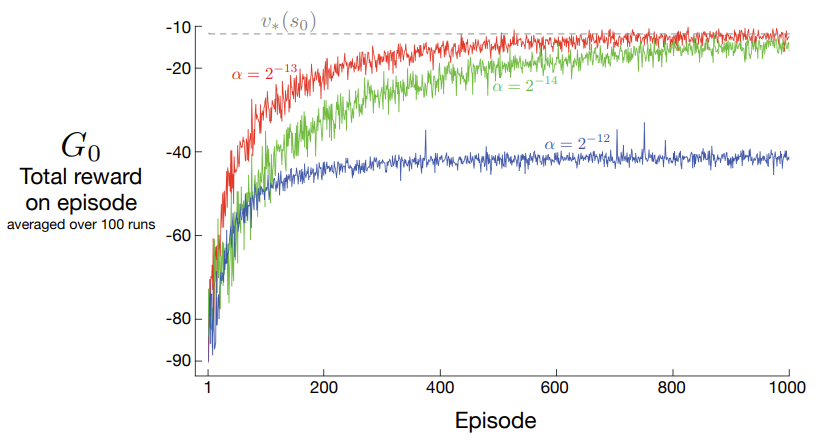
\includegraphics[width = 0.7\linewidth]{3.PNG}
    \caption{With a good step
size, the total reward per episode approaches the optimal value of the start state, shown in \cite{sutton2018reinforcement}.}
    \label{fig:stepsize}
\end{figure}

\begin{figure}[H]
    \centering
    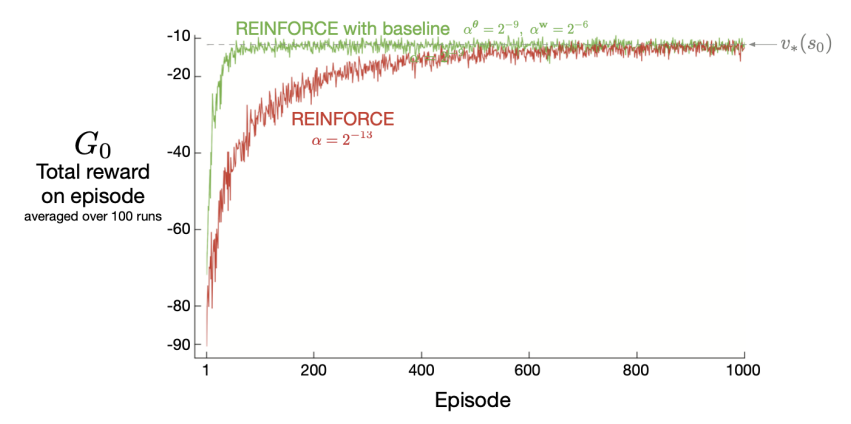
\includegraphics[width = 0.7\linewidth]{2.PNG}
    \caption{Adding a baseline to REINFORCE can make it learn much faster, shown in \cite{sutton2018reinforcement}.}
    \label{fig:converge}
\end{figure}




%This section provides any relevant background material that was not covered in the lectures, but was found to be useful for understanding the material. 
%For example, derivations, theory underlying techniques employed, etc. 

%Additionally, this section can summarizes applications or extensions of these techniques found in the literature. 

\end{document} % Done!